\documentclass{article}

\usepackage[shellescape]{gmp}
\usepackage[utf8]{inputenc}
\usepackage{german}

\usepackage{geometry}
\geometry{margin=1.5cm}

\usepackage{graphicx}
\DeclareGraphicsRule{*}{mps}{*}{}

\usepackage{pdflscape}

\usepackage{titling}
\setlength{\droptitle}{80px}

\renewcommand{\figurename}{Abbildung}
\begin{document}
\title{\Large Einsendeaufgabe UML}
\author{\normalsize Stefan Berger}
\date{}
\maketitle

\vspace{160px}

\listoffigures

\pagebreak

\hspace{0pt}
\vfill

\begin{figure}[h]
\centering
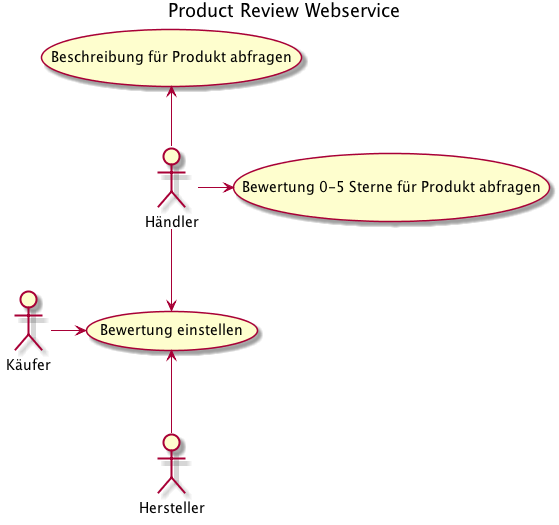
\includegraphics{mps/usecase.1}
\caption{Anwendungsfalldiagramm}
\end{figure}

\vspace{80px}

\begin{figure}[h]
\centering
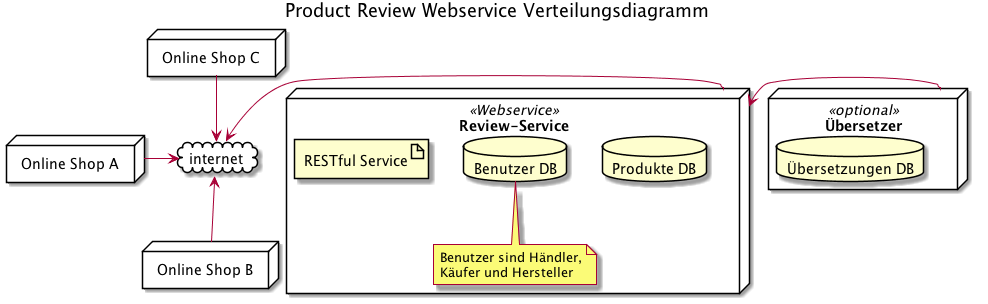
\includegraphics{mps/deployment.1}
\caption{Verteilungsdiagramm}
\end{figure}

\hspace{0pt}
\vfill

\pagebreak

\hspace{0pt}
\vfill
\begin{figure}[h]
\centering
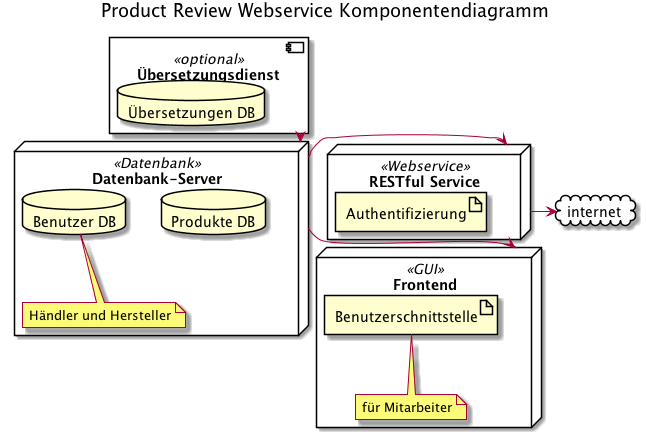
\includegraphics{mps/component.1}
\caption{Komponentendiagramm des Webservices}
\end{figure}

\vspace{80px}

\begin{figure}[h]
\centering
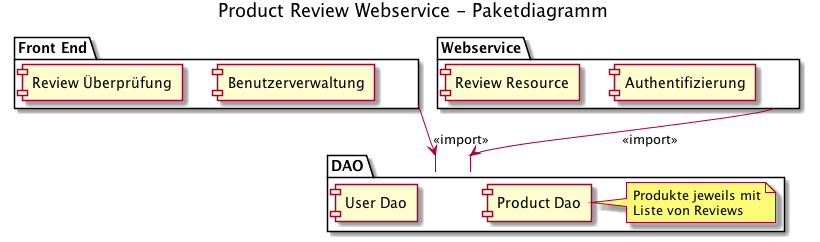
\includegraphics{mps/package.1}
\caption{Paketdiagramm des Webservices}
\end{figure}

\hspace{0pt}
\vfill

\pagebreak

\begin{landscape}
\begin{figure}[h]
\centering
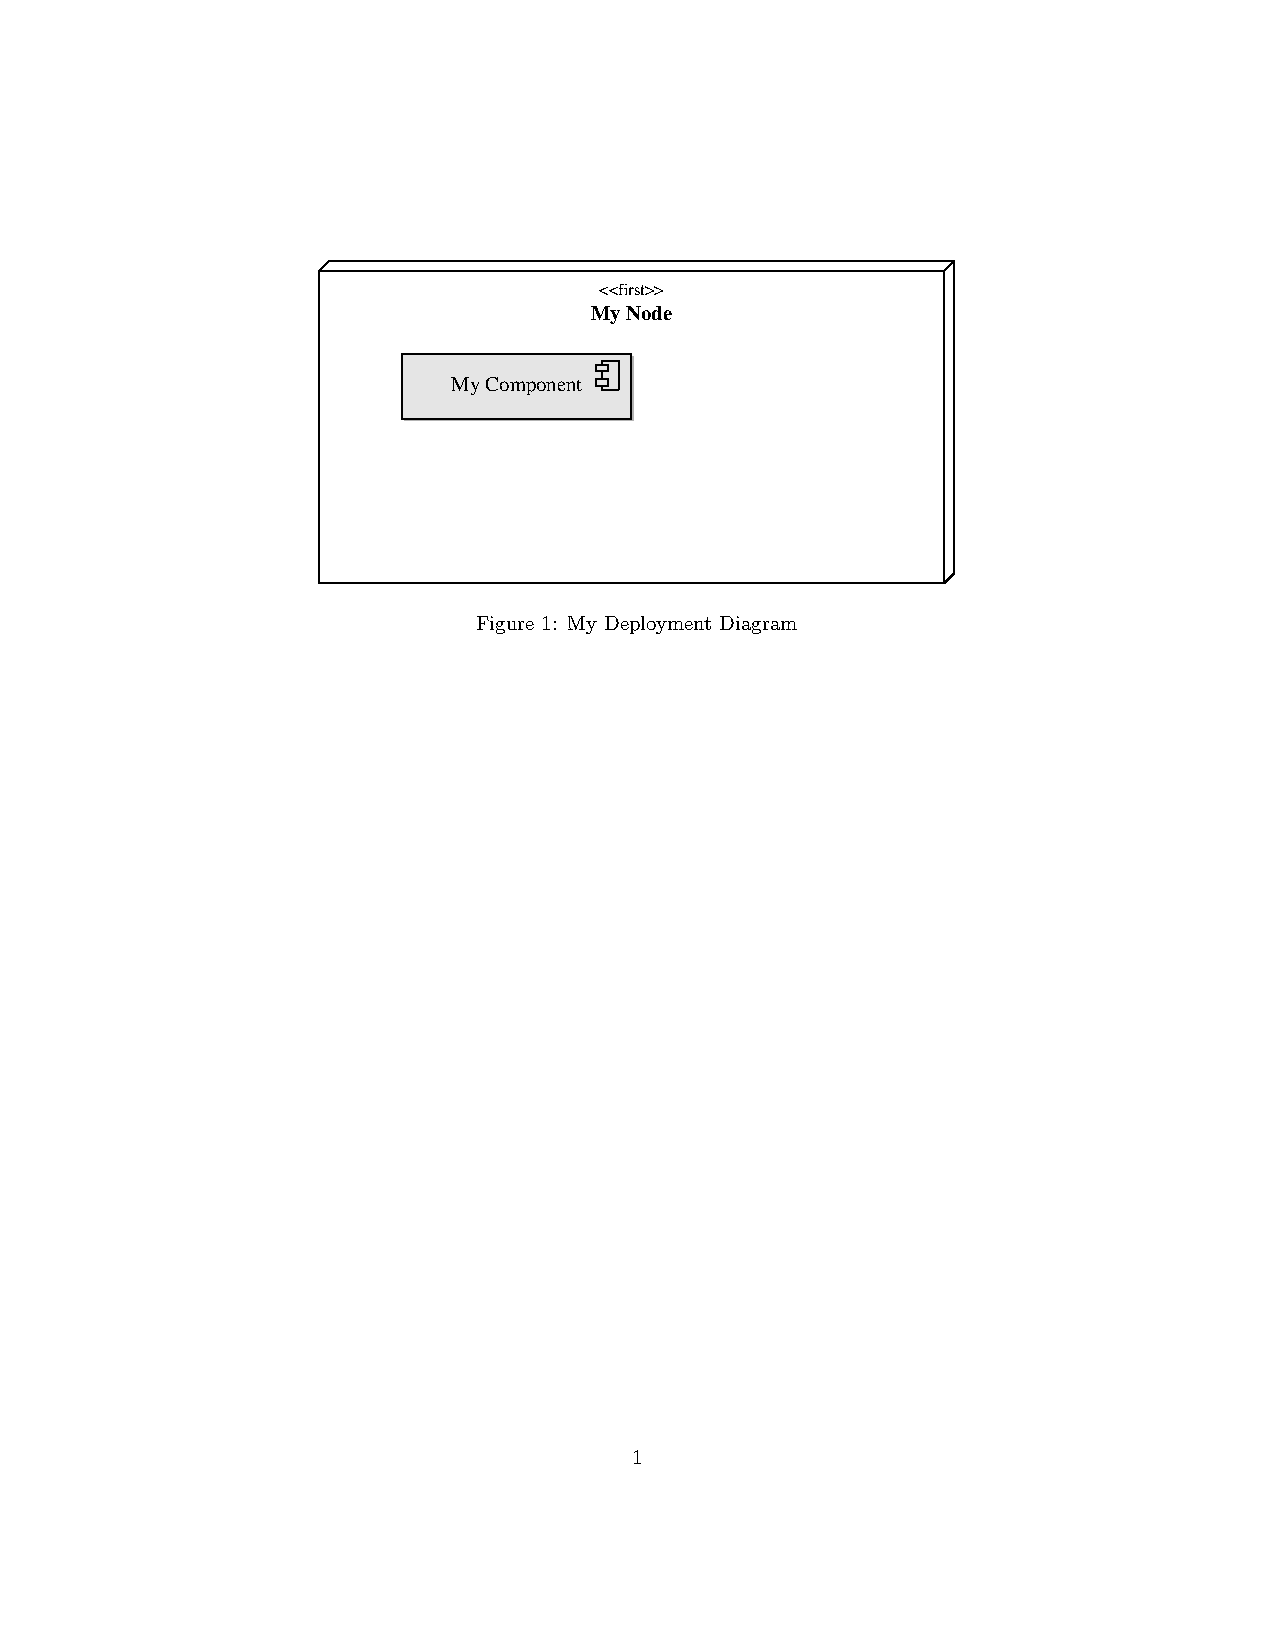
\includegraphics{mps/class.1}
\caption{Klassendiagramm}
\end{figure}
\end{landscape}

\pagebreak

\begin{landscape}
\hspace{0pt}
\vfill
\begin{figure}[h]
\centering
\includegraphics{mps/activity.1}
\caption{Aktivitätsdiagramm des Review-Prozesses (Lebenszyklus)}
\end{figure}
\hspace{0pt}
\vfill
\end{landscape}

\end{document}
